There always was a tight relation between the development of cameras and pixel detectors since 1969, when the idea of CCDs, thanks to whom Boyle and Smith were awarded the Nobel Prize in Physics in 2009, revolutionized photography allowing light to be captured electronically instead of on film. 
Even though the CMOS technology was already known when CCDs spread, the costs of productions were too high to allow the diffusion of these sensors for which needed to wait untill 1990s. From that period on, the fast diffusion of CMOS was mainly due to the less cost than CCD, and the less power required for supply. 

The principal use cases of pixel detectors are particle tracking and imaging: in the former case individual charged particles have to be identified, in the latter instead an image is obtained by the usually un-triggered accumulation of the impinging radiation. 
Also the demands on detectors performance depends on their usage, in particular tracking requires high spatial resolution, fast readout and radiation hardness. 


\section{Tracking in HEP}
    Historically, the first pixel detector employed in particle physics was a CCD: it was installed in the spectrometer at the CERN’s Super Proton Synchrotron (SPS) by the ACCMOR Collaboration (Amsterdam, CERN, Cracow, Munich, Oxford, RAL) at mid 1980s, with the pourpose of studing the recently-discovered charm particles.
    The second famous usage of CCDs took place at SLAC in the Large Detector (SLD) during the two years 1996-98. From that period on particle tracking in experiments have been transformed radically: it was mandatory for HEP experiments to build a inner vertex detector. 
    In 1991, the more demanding environments led to the development of hybrid pixel detectors: a dedicated collaboration, RD19, was established at CERN with the specific goal to define a semiconductor micropattern detector with an incorporated signal processing at a microscopic level. 
    In those years a wide set of prototypes of hybrid pixel has been manufactured; among the greatest productions a mention goes to the huge ATLAS and CMS vertex detectors. 
    From the middle of 2013 a second collaboration, RD 53, has been established with the new goal to find a pixel detector suitable for phase II future upgrades of those experiments. Even if the collaboration is specifically focused on design of hybrid pixel readout chips (aiming to \SI{65}{nm} tecnique so that the electronics fits within the pixel area), also other options have been taken in account and many test have been done on MAPS for example. Requirements imposed by HL-LHC will become tigher in time: for example, a dose and radiation of \SI{5}{Mrad} and \si{10 {16}}{NIEL} are exepcted after 5 years of operation. Time resolution, material budget and power consumption are also issues for the upgrade: a time resolution better than \SI{25}{ns} for a bunch crossing frequency of \SI{40}{MHz}, a material budget lower than 2\% and a power consuption lower than  \SI{500}{mW/cm\squared} are required. 

    Amidst the solutions proposed 3D silicon detector, invented by Sherwood Parker in 1995, and MAPS are the most promising. In 3D sensors the electrode is a narrow column of n-type implanted vertically across the bulk instead of being implanted on the wafer's surface. 
    The charge produced by the impinging particle is then drifted transversally within the pixel, and, as the mean path between two electrode can be soufficent low, the trap probability is not an issue. 
    3D pixels have been already proved in ATLAS tracker \red{quando?}. 
    Even if 3D detector are adequately radiation hard, MAPS architecture looked very promising from the beginning: they overcome both the CCDs long reading time and the hybrid problems (I have already explained in section \ref{sec:} the benefits of MAPS). 
    Experiments such as ALICE at LHC and STAR at RHIC have already introduced the CMOS MAPS technology in their detectors. ALICE Tracking System (ITS2), upgraded during the LHC long shut down in 2019-20, was the first large-area ($\sim$10 \si{m\squared} covered by 2.5 Gpixels) silicon vertex detector based on CMOS MAPS.

    \subsection{Hybrid pixels at LHC: ATLAS, CMS and LHC-b}
        \textbf{ATLAS}\\
        With CMS, ATLAS is one of two general-purpose detectors at the LHC and has the largest volume detector ever constructed for a particle
        collider (\SI{46}{m} long and \SI{25}{m} in diameter).  
        The Inner Detector consists of three different systems all immersed in a magnetic field parallel to the beam axis whose main components are: the pixel, the micro-strips and transition radiation trackers. Concerning the pixel detector, 92 million pixels are divided in 4 barrel layers and 3 disks in each end-cap region, covering a total area of \SI{1.9}{m\squared} and having a \SI{15}{kW} of power consumption.

        As stated by the ATLAS collaboration the pixel detector is exposed by an extreme particle flux: "By the end of Run 3\footnote{Run 3 start in June 2022}, the number of particles that will have hit the innermost pixel layers will be comparable to the number it would receive if it were placed only a few kilometres from the Sun during a solar flare". Considering that the particle density will increase even more with HL-LHC, radiation hardness is definitively target to achieve. 

        The most ambitious goal is employ a MAPS-based detector for the inner-layer barrels, and for this reason the RD53 collaboration is performing many test on MAPS prototypes, as Monopix of which I will talk about in section \ref{sec:}.
        
        Up to now this possibility will be eventualy implemented during the second phase of the HL-LHC era, as at the start of high-luminosity operation the selected option is the hybrid one. The sensor will be bonded with ITkPix, the first full-scale \SI{65}{nm} hybrid pixel-readout chip developed by the RD53 collaboration.
        Regarding the sensor, a valueable option is using 3D pixels, which have already proved themselves in ATLAS, for the insertable B layer (IBL).\red{qualcosa in più sui 3d.}
        The number of pixels will be increased of a factor about 7, passing from 92 milions to 6 billion.
    
        %3D silicon sensor technology has been chosen to instrument the innermost pixel layer of ITk, which is the most exposed to radiation damage. 50  50 and 25  100 .D
        %sensors are an established technology that has been already
        %employed in experiments at the LHC such as in the ATLAS
        %Insertable B-Layer (IBL)  and for the tracker of the AFP
        %experiment . With respect to these designs the new ITk 3D
        %sensors feature a reduced pixel cell size of 25  100 and 50 
        %50 um 2 with one collecting electrode .  active substrate of these new
        %sensors is reduced to 150 um in comparison to the previous
        %generation of 230 um thick 3D sensor
        \vspace{5mm}
        \textbf{CMS}\\

        \vspace{5mm}
        \textbf{LHCb} \\
        LHCb is a dedicated heavy-flavour physics experiment that exploits pp interactions at \SI{14}{TeV} at LHC. 
        It was the last experiment to upgrade the vertex detector, the Vertex Locator (VELO), replacing the silicon-strip with pixels in May 2022. 
        As the instantaneous luminosity in Run3 is increased by a factor $\lesssim$10, much of the readout electronics and of the trigger system have been developed in order to cope with the large interaction rate.
        To place the detector as close as possible to the beampipe and reach a better track reconstruction resolution, the VELO has a surprising feature: it can be moved. During the injection of LHC protons it is parket at \SI{3}{cm} from the beams and only when the stability is reach it is brought at $\sim$\SI{5}{mm}. Radiation hardness as well as readout speed are then a priority for the detectors: that's why the collaboration opted for a hybrid system. 
        The Velopix is made bonding sensors, each measuring 55 $\times$ 55 micrometers, \SI{200}{\um}-thick to a \SI{200}{\um}-thick ASIC specially developed for LHCb and coming from the Medipix family (sec. \ref{sec:}), which can handles hit rates up to \SI{900}{MHz} per chip.
        Since the detector is operated under vacuum near the beam pipe, the heat removal is particularly difficult and evaporative CO2 microchannel cooling are used. 

    \subsection{A DEPFET example: Belle-II}
        

    \subsection{CMOS MAPS: ALICE and STAR}
        \textbf{ALICE}\\
        ALICE (A Large Ion Collider Experiment) is a detector dedicated to heavy-ion physics and to the study of the condensed phase of the chromodynamics at the LHC.
        The tracking detector consists of the Inner Tracking System (ITS), the gaseous Time Projection Chamber (TPC) and the Transition Radiation Detector (TRD),  and all those are embedded in a magnetic field of \SI{0.5}{T}. The ITS is made by six layers of detectors, two for each type, from the interaction point outwards: Silicon Pixel Detector (SPD), Silicon Drift Detector (SDD) and Silicon Strip Detector (SSD).         
        Contrary to the others LHC experiments, ALICE tracker in placed in a quite different environments: the expected dose is smaller by two order of magnitude and the rate of interactions is few \si{MHz} instead of \SI{40}{MHz}, but the number of particles comes out of each interaction is higher (the SPS is invested by a density of particles of $\sim$\SI{100}{\per cm\tothe{-2}}).  
        The reconstruction of very complicated events whit a large number of particle is a challenge, hence to segment and to minimize the amount of material, which may cause secondary interaction complicating futher the event topology, is considered a viable strategy. 
        Thanks to the reduction of the material budget, ITS2, which uses the ALPIDE chip developed by ALICE collaboration, obtained an amazing improvement both in the position measurement and in the momentum resolution, improving the efficiency of track reconstruction for particle with very low transverse momentum (by a factor 6 at pT $\sim$ 0.1 GeV/c). Further advancements in CMOS MAPS technology are being aggressively pursued for the ALICE ITS3 vertex detector upgrades (foreseen around 2026-27), with the goals of further reducing the sensor thickness and improving the readout speed of the devices, while keeping power consumption at a minimum.\\
        \vspace{5mm}
        \textbf{STAR}\\
        MIMOSA-28 devices for the first MAPS-based vertex detector: a 356 Mpixel two-layer barrel system for the STAR experiment at Brookhaven’s Relativistic Heavy Ion Collide

\section{Applications in imaging}
    \red{frase introduttiva (?). Magari qualcosa tipo: Per l'imaging si possono usare o come integratori di carica (ad esempio si integra la carica rilasciata da più fotoni) oppure come contatori. In questo secondo caso l'utilizzo e l'elettronica utilizzata per leggerli assomiglia all'utilizzo agli acceleratori, anche se i requirements sono molto meno stringenti. Dato che l'utilizzo per l'imaging e per i tracciatori può non essere molto diverso, } two noteworthy of microchips originally meant for detectors in particle physics at the LHC, and later employed in other fields are Medipix and Timepix. They are read-out chips developed by the Medipix Collaborations since early 1990s. For two decades, different Medipix generations have been produced, having a rough correlation with the feature size used: Medipix2 (1999) used \SI{250}{nm} feature size CMOS while Medipix3 (2005) \SI{130}{nm}.
    The aim of the fourth collaboration (2016), instead, is designing pixel read-out chips that prepared for \red{TSV processing and may be tiled on all four sides. DOVREI METTERE DUE RIGHE SU TSV OPPURE TAGLIARE. }
    For photons imaging other materials with higher atomic charge than silicon could be prefered, as a high photon absorption efficiency is needed: it was for this reason that Medipix2 was bump bonded to identically segmented sensors of both silicon and GaAs.
    
    The applications in scientific imaging vary from atrophysics and medical imaging to more exotic domains as studies of protein dynamics, art authentication and dosimetry.
    The most important employment of Medipix is as X-ray single photon counting in industrial and medical radiography and in 3D computed tomography. 
    Thanks to a New-Zealand company, the MARS Bioimaging detector has been fabricated, which is capable of resolving the photons energy and produce 3D coloured images.
    Besides tracking in HEP (I have already cited the use of Timepix3 is in the beam telescope of the LHCb VELO),a important use of Timepix is in dosimetry \red{Timepix Detector for Imaging in Ion Beam Radiotherapy- aggiungi qualche info}
    A small-Timepix detector with the dimension of a USB can also be found at the International Space Statio, where it is exploited for radiation, principally made of haevy-ion, monitoring. 
 
    \subsection{Applicability to FLASH radiotherapy}
        \red{DA QUI IN POI IN QUESTO CAPITOLO CI SONO APPUNTI A CASO, DA RIORDINARE E TRADURRE}

        The radiological treatment is a commod method used in 60\% of tumors both as palliative care and as treatment. It can be given before, after or during a surgery, \red{per cosa sta iort} IORT. 
        Moreover many different types of radiations can be used to irradiate the affected tissues; high energy photons 

    Un problema dei fotoni ad esempio è che il loro rilascio di dose è lineare, per cui danneggi anche i tessuti sani. Il problema dei protoni invece è che hanno un picco troppo strtto per cui non puoi coprire grosse zone e sorpattuto se sbagli rischi davvero di danneggiare moooolto i tessuti sani.\\

    Curva di efficacia del trattamento in funzione della dose:
    The surviving fraction probability is de
    \begin{equation}
        \frac{S(D)}{S(0)}=e^{-F(D)}
    \end{equation} 
    dove F(D)   
    \begin{equation}
        F(D) = \alpha D + \beta D^2
    \end{equation} 
    dove $\alpha$ e $\beta$ rappresentano due tipi di danno diversi: coefficients, experimentally determined, characterizing the
    radiation response of cells. In particularly, alpha represents the rate of cell killing
    by single ionizing events, while beta indicates the maximal rate of cell killing by
    double hits observed when the repair mechanisms do not activate during the
    radiation exposure.
    Si ottiene una curva di sopravvivenza dove si vede la possibilità delle cellule di autoripararsi. A basse dosi infatti le cellule possono ripararsi.\\

    Per introdurre l'effetto FLASH instroduco prima la therapeutic window.  \\

    \begin{figure}
        \centering
        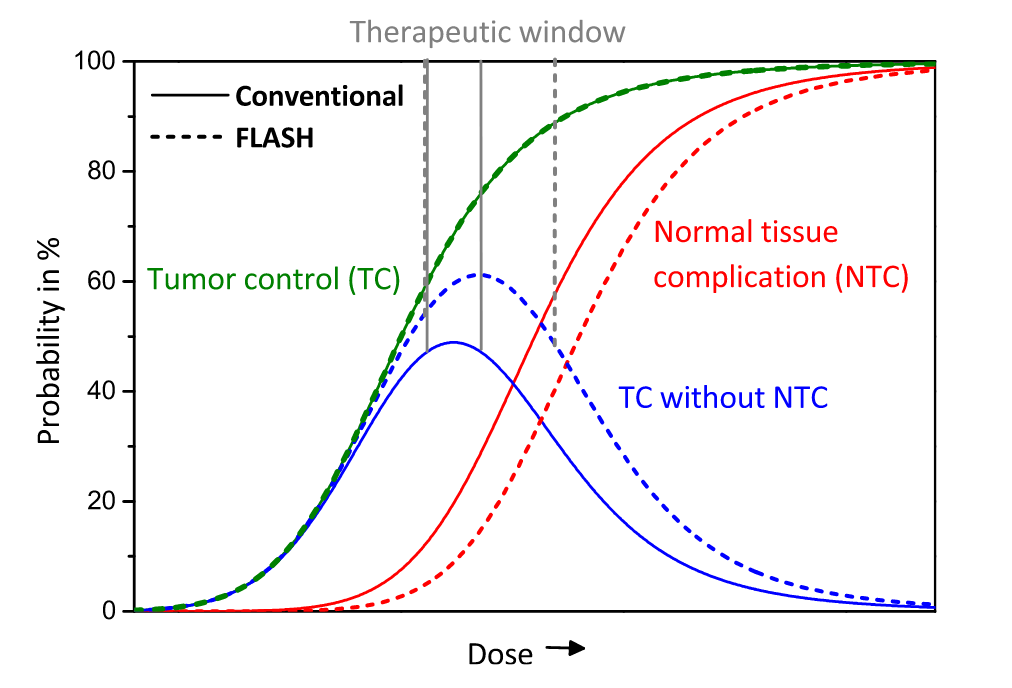
\includegraphics[width=.8\linewidth]{figures/pixel_detectors_usage/curve_flash.png}
        \caption{}
        \label{fig:}
     \end{figure}
    
    TCP è la tumor control Probability che indica la probabilità delle cellule del tumore di essere uccise dopo una certa dose (con in riferimento a dose in acqua)\\
    Se una media di $\mu(D)$ di cellule di tumore are killed con una dose D, la probabilità che n cellule sopravvivono è data da $P(n|\mu)$ poisson:
    \begin{equation}
        P(n|\mu) = \frac{\mu(D)^ne^{-\mu(D)}}{n!}
    \end{equation}    

    \begin{equation}
        TPC(D) = P(n=0|\mu(D))= e^{-\mu(D)}
    \end{equation} 
    D'altra parte hai una probabilità di fare danno su normal tissue NTCP Normal Tissue Complication Probability, che rappresenta il problema principale e che limita la massima radiazione erogabile\\
    Una scelta bilanciata si applica guardando a questi due fattori; si usa il therapeutic index definito come TCP/NTCP.\\
    La cosa ottimale è ampliare la finestra del therapeutic ratio.\\


    CONV-RT 0.01-5 Gy/min. A typical RT regime today consists of daily franctions of 1.5 to 3 Gy given over several weeks.\\
    Nell Intra operative radiation therapy (IORT), where they reach values respectively about
    20 and 100 times greater than those of conventional radiation therapy.

    FLASH vuole ultrahigh mean dose-rate (maggione di 40 Gy/s) in modo da ridurere anche il trattamento a meno di un secondo. \\


    Ci sono due effetti che affect the flsh effect and la sua applicabilità: Dose rate effect e oxygen\\
    \begin{itemize}
        \item dose rate effect
        \item oxygen effect
    \end{itemize}    

    Cellule che esibiscono hypoxia (cioè cellule che non hanno ossigeno sono radioresistenti); al contrario normoxia e physoxia non lo sono.
    la presenza di ossigeno rende la curva steeper indicando che lo stesso danno si raggiunge a livelli di dose più bassi rispetto al caso senza ossigeno.\\
    FIGURA con una curva a confronto con e senza ossigeno.\\
    Typically, the OER is in the order of 2.5-3.5 for most cellular systems


    Quindi si vogliono sfruttare questi effetti per diminuire la tossicità sui tessuti sani\\




